\documentclass[a4paper,french,12pt]{report}
\usepackage[utf8]{inputenc} % Encodage du fichier
\usepackage[T1]{fontenc} % Encodage des fonts nécessaire pour le Latin
\usepackage[english,frenchb]{babel} % Pour changer la langue des mots générés et choisir la bonne mise en page
\usepackage{lmodern} % Le latin modèrne
\usepackage[top=2cm, bottom=2cm, left=3cm, right=2cm]{geometry} % Définir les marges de la page
\usepackage{amsmath} % Pour des fonctions mathématiques
\usepackage{amssymb} % Pour les symbols mathématiques
\usepackage[hidelinks]{hyperref} % Pour les liens
\usepackage{fancyhdr} % Pour le style de la page
\usepackage[font=it]{caption} % Rendre les titres des tableaux italiques
\usepackage{microtype}
\usepackage{graphicx} % Pour les images
\usepackage{subcaption} % Pour mettre plusieurs images sur la même ligne
\usepackage{float} % Pour empêcher le déplacement des tableaux et des figures.
\usepackage[french,longend,boxruled,algoruled,linesnumbered,algochapter]{algorithm2e}%pour les algorithmes
\newcommand\mycommfont{\footnotesize\ttfamily\textcolor{blue}}%pour colorer les commenataires en bleu
\usepackage{babelbib} % Pour changer la langue dans la bibliographie
\usepackage{amsthm} % Pour les exemples
\usepackage{xspace}

\graphicspath{ {pictures/} } % Spécifier le répertoire contenant les images  
\DisableLigatures[f]{encoding=*}
\renewcommand \thechapter{\Roman{chapter}} % Utiliser la numéros romans pour les chapitre
\AtBeginDocument{% Changer "Table"
  \renewcommand\tablename{\itshape Tableau}
  \renewcommand{\figurename}{\itshape Figure}
	% Renommer la table des matières
	\renewcommand{\contentsname}{Sommaire}
}


\date{}
% Style de l'entête et le pied de la page 
\setlength{\headheight}{16pt}
\pagestyle{fancyplain}
\lhead{} % Enlever la section
\rhead{\fancyplain{}{\footnotesize \itshape{\nouppercase{\leftmark}}}} % Titre du chapitre en miniscule avec taille 10
\cfoot{} % Déplacer le numéro de la page
\rfoot{\fancyplain{\thepage}{\thepage}} % à droite de la page

% Espace entre les lignes
\linespread{1.3}
% Nom de notre application
\newcommand{\appname}{\textbf{combinateur d'évidences}\xspace}
\newcommand{\appName}{Combinateur d'évidences\xspace}
% Nom de la grande interface
\newcommand{\platformename}{\textbf{plateforme d'outils SII}\xspace}
\newcommand{\platformeName}{Plateforme d'outils SII\xspace}

% Gérer les exemples
\theoremstyle{definition}
\newtheorem{exemple}{Exemple}

\begin{document}
\newpage
\begin{titlepage}
\begin{center}
\section*{\textit{Remerciements}}
\end{center}
\textit{
\subparagraph{}
Tout d’abord, louange à « Allah » qui nous a guide sur le droit chemin tout au long du travail et nous a inspiré les bons pas et les justes reflexes. Sans sa miséricorde, ce travail n’aura pas abouti.
\subparagraph{}
Nous tenons à exprimer notre profonde reconnaissance au Madame Hadja Faiza Khellaf-Haned pour son encadrement, ces nombreux conseils et son soutien constant tout au long de notre Mémoire. Nous la remercions chaleureusement d’avoir encadré ce travail de Licence, avec beaucoup de compétence, d’enthousiasme et de disponibilité.
\subparagraph{}
Nous tenons à exprimer notre gratitude au Madame Khaoula Boutouhami pour nous avoir fait profiter de son expérience de recherche dans le domaine. Ses conseils sur l’aspect théorique et pratique qui nous ont été utiles et permis de mener à bien cette thèse.
\subparagraph{}
Nous remercions Mesdames A.Mokhtari, A.Akli d’avoir accepté de faire partie de notre jury de Licence. Nous leur exprimons notre profonde gratitude.
\subparagraph{}
Nous remercions tous les chercheurs, enseignants et membres du personnel de notre département d’informatique pour, nous avoir aidé pendant ces trois années d’études.
\subparagraph{}
Nous tenons à remercier  également tous  nos  amis, qui nous ont aidés au cours des trois années de notre parcours.
\subparagraph{}
Enfin, nous remercierions jamais assez nos parents nos frères et soeurs pour le soutien sans faille et permanent durant ces années, qui l'accomplissement de ce mémoire n'aurait pas eu lieu dans ces délais. Ils étaient là pour nous.
Nous tenons à leur dédier ce mémoire. 
}
\thispagestyle{empty}
\end{titlepage}
\tableofcontents
\listoffigures
\listofalgorithms
\parskip=0.6em


\phantomsection
\addcontentsline{toc}{chapter}{Introduction générale}
\chapter*{Introduction générale}

Notre projet traite un sujet dans le domaine de l'intelligence artificielle. Il est dans le but de la
manipulation des connaissances incertaines.

Il est composé à partir de deux parties principales. D'abord, il sagit de réaliser un logiciel complet qui
implémente une des théories de ce domaine connue sous le nom de \emph{la théorie de Dempster-Shafer}. Ensuite,
il est dans l'objectif de créer une plateforme permettant de regrouper plusieurs outils dont le rôle de chaque outil est de
résoudre un problème d'incertain. Cette plateforme facilite l'utilisation de ces outils en offrant une interface
commune pour les exploiter.

Ce projet répond aux besoins des étudiants du Master 2 de la spécialité SII \footnote{Systèmes Informatiques Intelligents}
de notre département, dans leurs séances de TP. Il a comme but de compléter le manque d'un logiciel pour
effectuer les grands calculs requis par l'application de la théorie de Dempster-Shafer pour résoudre un
problème donné. En plus, il offre une interface pour tout les outils que les étudiants ont l'habitude de les utiliser.

Dans le premier chapitre nous expliquerons les concepts de la théorie de Dempster-Shafer et les règles de combinaison
et de décision associées. Dans le deuxième, nous parlons sur les théories de l'incertain qui sont implémentées
par les outils exploités à travers la plateforme. Dans le chapitre qui suit nous présentons quelques algorithmes que
nous avons conçu et implémenté dans notre logiciel. Enfin, le dernier chapitre est consacré pour la présentation de ce que
nous avons réalisé.
\parskip=0.6em
\chapter{Théorie de Dempster and Shafer}

\phantomsection
\addcontentsline{toc}{section}{Introduction}
\section*{Introduction}

La théorie de Dempster-Shafer, également connue comme la théorie de l'évidence,
ou théorie des fonctions de croyance, est une théorie mathématique du raisonnement
sur l’évidence et la plausibilité. Elle a été développée par Glenn Shafer (1976)
en se basant sur des travaux antérieurs de Arthur Dempster (1968). Elle a attiré
l’attention des chercheurs de l'intelligence artificielle au début des années 80.

Dans un espace discret fini, la théorie de Dempster-Shafer représente la généralisation
de la théorie des probabilités dans laquelle les probabilités sont assignées à des ensembles,
contrairement aux singletons mutuellement exclusifs.

\section{Concepts de base}

\subsection{Quelques notations}

Nous allons présenter ici les conventions de notation utilisées dans la suite de ce mémoire.

Soit $\Omega$ un univers constitué d'un ensemble fini qui contient toutes les propositions
auxquelles on s'intéresse, appelé également cadre de discernement. On note $\varnothing$
l’ensemble qui ne contient aucun élément de $\Omega$. $\mathcal{P}(\Omega)$ représente
l’ensemble contenant toutes les parties (les sous-ensembles) de $\Omega$. On note aussi
les opérations binaires sur les ensembles $\subset$, $\cup$ et $\cap$, qui sont l’inclusion,
l’union et l’intersection, respectivement. On appelle hypothèse un élément de $\mathcal{P}(\Omega)$.

La théorie de Dempster-Shafer est caractérisée par trois fonctions principales :
\textbf{l’assignement de probabilité de base} (\emph{basic probability assignement bpa}),
\textbf{la croyance} (\emph{belief}) et \textbf{la plausibilité} (\emph{plausibility}).

\subsection{L’assignement de probabilité de base}

Appelé aussi la fonction de masse, noté $m$, c'est une fonction qui affecte le degré d’évidence
disponible à un élément $A$, et seulement à $A$, de $\mathcal{P}(\Omega)$ dans l’intervalle
$[0,1]$, tel que les $m(A)$ s’additionnent à $1$.

$m(\varnothing)$ --qui représente l’absence
de solution-- est toujours égale à $0$ car $\Omega$ doit être exhaustive, et la somme de $m(A)$
vaut $1$. Chaque élément A tel que $m(A) > 0$ est appelé élément focal.

Généralement, le bpa n’est pas un équivalent de la fonction de probabilités classique. En effet,
la valeur exacte de la probabilité (dans le sens classique) appartient à un intervalle borné par
deux valeurs qui sont \emph{la croyance} et \emph{la plausibilité}.

Formellement, on peut représenter cela par :
\begin{equation}
m : \mathcal{P}(\Omega) \mapsto [0,1]
\end{equation}
\begin{equation}
m(\varnothing) = 0
\end{equation}
\begin{equation} \label{somme_masses}
\sum_{A \in \mathcal{P}(\Omega)} m(A) = 1
\end{equation}

\subsubsection{Exemple}
Dans une enquête sur un incident de vol, trois personnes \textit{P1}, \textit{P2}, \textit{P3}
sont accusées. L’enquêteur pense à 30\% que P1 est le voleur, à 50\% que l’un des deux autres
personnes P2 ou P3, est le voleur, et à 10\% que P1 ou P3 le soit.\\
Le cadre de discernement s'écrit ainsi : $$\Omega = \{P1, P2, P3\}.$$
L'ensemble de parties de $\Omega$ est : $$\mathcal{P}(\Omega) = \{\varnothing, \{P1\}, \{P2\},
\{P3\}, \{P1, P2\}, \{P1, P3\}, \{P2, P3\}, \Omega\}$$
La distribution des masses s'exprime ainsi : $$m(\{P1\}) = 0.3, m(\{P2, P3\})  = 0.5,
m(\{P1, P3\}) = 0.1$$ et $$m(\Omega) = 1 - (0.3+0.5+0.1) = 0.1$$ à partir de l’équation \ref{somme_masses}.\\
Les masses des hypothèses restantes sont toutes égalles à $0$.

\subsection{La croyance}

La croyance est la quantité de confiance qui supporte une hypothèse $A$ de
$\mathcal{P}(\Omega)$, toutes parties comprises.\\
On la note $Cr(A$) ou plus souvent $Bel(A)$. Il est clair que $Bel(\varnothing)$
est nulle, et $Bel(\Omega)$ est toujours 1. Il faut noter que la croyance est une
mesure non additive, c’est-à-dire que $Bel(A) + Bel(\Omega - A) \neq 1$.

Formellement :
\begin{equation}
Bel(\varnothing)=0
\end{equation}
\begin{equation}
Bel(\Omega)=1
\end{equation}
\begin{equation}
Bel(A) = \sum_{B \slash B \subseteq A} m(B)
\end{equation}
\begin{equation}
\forall p,q \in \mathcal{P}(\Omega) \medskip Bel(p \cup q) \geq Bel(p) + Bel(q) - Bel(p \cap q).
\end{equation}
On peut aussi obtenir le bpa avec la fonction inverse suivante :
\begin{equation}
m(A) = \sum_{B \slash B \subseteq A} (-1)^{|A-B|} Bel(B),
\end{equation}
où $|A-B|$ est la différence des cardinalités entre les deux ensembles.

\subsubsection{Exemple}
En continuité de l'exemple précédent, on calcule la croyance de chaque hypothèse :

\begin{table}[h!]
\centering
\begin{tabular}{|l|l|}
\hline
Hypothèse $A$ & Croyance $Bel(A)$\\
\hline
$\varnothing$ & $0$ \\
\hline
$\{P1\}$ & $0.3$ \\
\hline
$\{P2\}$ & $0$ \\
\hline
$\{P3\}$ & $0$ \\
\hline
$\{P1, P2\}$ & $0.3 + 0 + 0 = 0.3$ \\
\hline
$\{P1, P3\}$ & $0.3 + 0 + 0.1 = 0.4$ \\
\hline
$\{P2, P3\}$ & $0 + 0 + 0.1 = 0.1$ \\
\hline
$\Omega$ & $1$ \\
\hline
\end{tabular}
\caption{Les croyances calculées à partir de la distribution de masses}
\end{table}

\subsection{La plausibilité}

La plausibilité représente la croyance qu’il est possible
d’affecté à une hypothèse $A$ de $\mathcal{P}(\Omega)$; autrement dit,
c’est la croyance affectée à A et aux hypothèses dont l'intersection
avec $A$ n’est pas vide. On la note $Pl(A)$. La valeur de la plausibilité est
toujours supérieure ou égale à celle de la croyance. Identiquement à la
croyance, $Pl(\varnothing)$ est nulle, et $Pl(\Omega)$ vaut $1$.

Formellement :
\begin{equation}
Pl(\varnothing) = 0
\end{equation}
\begin{equation}
Pl(\Omega) = 1
\end{equation}
\begin{equation}
Pl(A) = \sum_{B \slash B \cap A \neq \varnothing} m(B)
\end{equation}
La plausibilité peut aussi être dérivée à partir de la croyance:
\begin{equation}
Pl(A) = 1 - Bel(\bar{A}),
\end{equation}
où $A$ est le complément de $A$ dans $\Omega$.

La probabilité classique d’un événement $A$, $P(A)$ est représentée par
l’intervalle qui a comme bornes inférieure et supérieure $Bel(A)$ et $Pl(A)$,
respectivement, c’est-à-dire $$Pl(A) \leq P(A) \leq Bel(A).$$
Si $$Bel(A) = Pl(A),$$ alors la probabilité de $A$ est unique et $$P(A) = Bel(A) = Pl(A)$$

\subsubsection{Exemple}
On calcule les plausibilités pour le même exemple.

\begin{table}[h!]
\centering
\begin{tabular}{|l|l|}
\hline
Hypothèse $A$ & Plausibilité $Pl(A)$\\
\hline
$\varnothing$ & $0$ \\
\hline
$\{P1\}$ & $0.3 + 0.1 + 0.1 = 0.5$ \\
\hline
$\{P2\}$ & $0.5 + 0.1 = 0.6$ \\
\hline
$\{P3\}$ & $0.5 + 0.1 + 0.1 = 0.6$ \\
\hline
$\{P1, P2\}$ & $0.3 + 0.5 + 0.1 + 0.1 = 1$ \\
\hline
$\{P1, P3\}$ & $0.3 + 0.5 + 0.1 + 0.1 = 1$ \\
\hline
$\{P2, P3\}$ & $0.5 + 0.1 + 0.1 = 0.7$ \\
\hline
$\Omega$ & $1$ \\
\hline
\end{tabular}
\caption{Les plausibilités calculées à partir de la distribution de masses}
\end{table}
\section{Règles de combinaison}

Souvent, on obtient l’information à partir de sources distinctes et indépendantes,
et généralement ces sources ne sont pas parfaites, c’est pourquoi on a besoin de
fusionner les évidences fournies par ces sources en utilisant des règles de
combinaison. Il existe trois types de combinaison : \emph{conjonctive},
\emph{disjonctive}, et \emph{mixte}.

\subsection{Combinaison conjonctive}

Dempster a introduit une règle connue sous le nom de règle de combinaison
de Dempster (\emph{Dempster's Combination Rule}) pour fusionner deux pièces
d’évidence qui peuvent être représentées par deux fonctions de croyance.Cette
règle respecte les quatre propriétés algébriques suivantes : l’associativité,
la commutativité, l’idempotence et la continuité.

Soient deux fonctions de masse $m_1(A)$ et $m_2(A)$ associées à deux fonctions
de croyance $Bel_1(A)$ et $Bel_2(A)$ respectivement. $(Bel_1 \oplus Bel_2)(A)$
est définie à travers la masse $m_{1 \oplus 2}(A)$ :
\begin{equation}
m_{1 \oplus 2}(A) = \sum_{B \cap C = A} m_1(B) m_2(C).
\end{equation}

Néanmoins, cette règle a été critiquée par de nombreux chercheurs, parce qu’elle
n’est pas normalisée. En d’autre termes, elle permet d’affecter des masses à
des ensembles vides. Ce problème est dû au fait que l’intersection de deux
éléments focaux peut générer $\varnothing$, ce qui dénote un conflit entre les croyances.

Pour corriger ce problème, Shafer a proposé d’ignorer carrément les conflits
et d'étendre la distribution des masses. Le facteur de conflit est une valeur
$K < 1$ et définie par :
\begin{equation}
K = \sum_{B \cap C = \varnothing} m_1(B) m_2(C).
\end{equation}

Afin de normaliser la distribution de masse, la règle de Dempster doit être
multipliée par la quantité $(1 - K)^{-1}$. Donc la règle de Dempster-Shafer
est représentée par les équations suivantes :
\begin{equation}
m(\varnothing) = 0
\end{equation}
\begin{equation}
m(A) = \frac{1}{1-K} \sum_{B \cap C = A \neq \varnothing} m_1(B) m_2(C)
\end{equation}

Cependant, la règle de Shafer n’est pas toujours satisfaisante à cause de la
normalisation qui considère que le conflit vient de l’imperfection des sources.

D’autres chercheurs ont proposé des règles différents, comme Smets qui a introduit
une forme non normalisée pour prendre en compte les univers ouverts. Il suppose
que le conflit vient du fait que l’ensemble $\Omega$ n’est pas exhaustif. Pour
cette raison, la règle de Smets affecte une masse $K$ à $\varnothing$ qui représente
une hypothèse manquante. Elle est définie par ces équations :
\begin{equation}
K = m(\varnothing) = \sum_{B \cap C = \varnothing} m_1(B) m_2(C)
\end{equation}
\begin{equation}
m(A) = \sum_{B \cap C = A \neq \varnothing} m_1(B) m_2(C)
\end{equation}

Par contre, Yager propose un modèle d’un univers fermé ($\Omega$ est exhaustif).
La mesure de conflit est ajoutée à la mesure du cadre de discernement $\Omega$.
Donc le conflit sera transformé en ignorance. On obtient ces équations :
\begin{equation}
m(\varnothing) = \sum_{B \cap C = \varnothing} m_1(B) m_2(C)
\end{equation}
\begin{equation}
m(\Omega) = \left(1 - \sum_{A \in \mathcal{P}(\Omega)}
\sum_{B \cap C = A \neq \varnothing} m_1(B) m_2(C)\right) +
\sum_{B \cap C = \varnothing} m_1(B) m_2(C)
\end{equation}

\subsection{Combinaison disjonctive}

Dans la combinaison disjonctive on considère l’utilisation de l’union à la place
de l’intersection. Les éléments focaux sont obtenus à partir de la table d’union.
La fonction de masse de la règle de combinaison disjonctive est formalisée par l'équation :
\begin{equation}
m(A) = \sum_{B \cup C = A \neq \varnothing} m_1(B) m_2(C).
\end{equation}

Comme l’union de deux éléments focaux ne peut être jamais vide, on est sûr
que $m(\varnothing)=0$. Cela veut dire qu’il est impossible d’obtenir un conflit
lors de la combinaison. En contrepartie, l'union peut causer une perte de spécificité
vu que les masses sont élargies. Cette approche apparaît plus intéressante en
l’absence des informations nécessaires sur la fiabilité des sources.

\subsection{Combinaison mixte}

Dubois et Prade ont proposé une combinaison mixte comme un compromis entre la
combinaison conjonctive et la combinaison disjonctive et comme un essai de conserver
les avantages des deux. De même que la combinaison de Yager, le modèle de Dubois
et Prade suppose que le conflit est dû à la non fiabilité des sources. La règle de
Dubois et Prade est définie comme suit :
\begin{equation}
m(A) = \sum_{B \cap C = A \neq \varnothing} m_1(B) m_2(C) +
\sum_{\substack{B \cup C = A \neq \varnothing \\ B \cap C = \varnothing}} m_1(B) m_2(C)
\end{equation}

\section{Décision}

Prendre une décision veut dire choisir une hypothèse élémentaire parmi les autres
par la maximisation d'un critère. La sélection est établie en observant
la croyance et la plausibilité de chaque hypothèse résultante. Il existe trois règles
de décision : le \emph{maximum de croyance}, le \emph{maximum de plausibilité} et le
\emph{maximum de probabilité pignistique}

\subsection{Maximum de croyance}

Dans cette règle on s'intéresse à trouver l'hypothèse élémentaire $\omega_i$ qui
a la croyance maximale. C'est-à-dire que $\omega_i$ est choisie si elle satisfait cette
équation :
\begin{equation}
Bel(\omega_i) = \max_{1 \leq j \leq n} Bel(\omega_j)
\end{equation}
Cette méthode est connue par son caractère très pessimiste.

\subsection{Maximum de plausibilité}

En opposition à la règle précédente, l'élément $d_i$ est sélectionné par le maximum
de plausibilité. En d'autres termes, on choisit le $d_i$ qui résoud cette équation :
\begin{equation}
Pl(\omega_i) = \max_{1 \leq j \leq n} Pl(\omega_j).
\end{equation}
Ainsi, cette méthode a un caractère très optimiste.

\subsection{Maximum de probabilité pignistique}

Cette règle est proposée par Smets et Kennes. Elle consiste à transformer la fonction
de masse $m(A)$ en une fonction de probabilité $BetP(\omega)$. Cette transformation
est appelée \emph{transformation pignistique} et définie par cette équation :
\begin{equation}
BetP(\omega) = \sum_{\substack{A \subseteq \Omega \\
\omega \in A}} \frac{1}{|A|}  \frac{m(A)}{1-m(\varnothing)}.
\end{equation}

Dans cette transformation, la masse de croyance $m(A)$ est distribuée uniformément
sur l’ensemble des éléments de $A$. Le critère est de prendre l'élément qui a le
maximum de probabilité pignistique. On peut voir cette méthode comme un compromis
entre les deux précédentes.

\phantomsection
\addcontentsline{toc}{section}{Conclusion}
\section*{Conclusion}

Après cette présentation de la théorie des fonctions de
croyances, des règles de combinaisons qui peuvent si appliquer,
et des règles de décisions compatibles, nous allons maintenant pouvoir introduire
des notions sur les théories de l'incertain.
\parskip=0.6em
\chapter{Les théories de l'incertain}

\phantomsection
\addcontentsline{toc}{section}{Introduction}
\section*{Introduction}



\section{L’incertain}

Les approches logiques de l’incertain permettent d’utiliser un langage formel pour la description des connaissances et le raisonnement automatique. Elles constituent une référence aux autres formalismes surtout pour le raisonnement, néanmoins les connaissances ne  sont pas structurées.

les principales représentations des connaissances incertaines sont le mode logique et le mode graphique.
Sur le plan de la représentation le mode graphique est le plus explicite en soumettant les relations de dépendances qui existe entre les différentes variables .sur le plan de résonnement, le mode logique offre une machinerie d’inférence efficace.

Plusieurs chercheurs ont permis l’émergence d’un certain nombre de modèles graphiques offrant un cadre de représentation plus structuré.

La théorie des possibilités est une théorie de l’incertain ayant pour vocation de manipuler des connaissances incomplètes. Elle diffère de la théorie de probabilité  vu quelle manipule deux mesures duales : possibilité et nécessité. Cette théorie a été développée dans deux directions : qualitative et quantitative ceci permet en fait de définir deux types de réseaux causaux possibilistes : les réseaux causaux possibilistes basé sur le minimum (qualitatif) et une autre base sur le produit (quantitative).



\subsection{Théorie de probabilité(BNT)}

La théorie des réseaux bayésien peut être considérée comme une fusion de diagrammes d'incidence et le théorème de Bayes. La probabilité qu'un événement se produise étant donné que un autre événement a déjà eu lieu est appelé une probabilité conditionnelle. 

Un réseau bayésien une représentation probabiliste des relations incertaines, qui se est avéré être utile pour la modélisation de problèmes du monde réel .Le modèle probabiliste est décrit qualitativement par un graphe acyclique orienté, ou DAG (Directed Acyclic Graph). Les sommets du graph représentent des variables, les arcs représentent la dépendance entre les variables. Le réseau comprennent aussi un ensemble de tables de probabilités, en indiquant les probabilités pour les vrais / fausses valeurs des variables.

Les avantages du  modèle graphique est qu’un réseau bayésien peut être utilisé pour apprendre les relations causales, et peut donc être utilisé pour obtenir la compréhension d'un domaine de problème et de prévoir les conséquences de l'intervention.

Ce que le champ a manqué est un logiciel à usage général correspondant. C’est pour cela la tentative de construire un tel paquet, appelé le Bayes Net Boîte à outils (BNT).

Une des plus grandes forces de BNT est qu'il offre une variété d'algorithmes d'inférence, chacun fait différents métiers entre la précision, de la généralité, la simplicité, la vitesse, etc.


\subsection{Théorie de possibilité quantitative}

\subsubsection{Graphique}

Un graphe possibiliste basé sur le produit (quantitatif), noté par GP P, est un graphe possibiliste ou les possibilités conditionnelles sont obtenues par le conditionnement de type produit. La distribution de possibilité des réseaux possibilistes bases sur le produit, notée par Pi P, est obtenue par la règle de chaınage 
pi P (V1, .., VN) = PRODi=1..N pi (Vi/PARVi).
 	
Ou PROD est l’opérateur produit.
La Boîte à outils PNT possède de différents algorithmes pour les réseaux causaux possibilistes basée sur le produit à connexions multiples et pour les polyarbres. 
\subsubsection{Logique}

La logique possibiliste offre un cadre générale pour représenter les connaissances incertaines, en terme de formules logiques classique auxquelles sont associé des pondérations appartenant à une échèle linaire [0,1].
\subsection{Théorie de possibilité qualitative}
\subsubsection{Graphique}

Un graphe possibiliste basé sur le minimum, noté par GPM, est un graphe possibiliste ou les possibilités conditionnelles sont obtenues par le conditionnement minimum. La distribution de possibilité des réseaux possibilistes basée sur le minimum, notée par pi M, est obtenue par la règle de chainage :
 pi M (A1, .., AN) = MINi=1..N pi (Ai/teta Ai) 
Ou MIN est  l’opérateur minimum.

La Boite à outils PNT possède aussi de différents algorithmes pour les réseaux causaux possibilistes basée sur le minimum à connexions multiples et pour les polyarbres. 
\subsubsection{Logique}



\subsection{Décision dans l’incertain}
\subsubsection{Graphique}

\subsubsection{Logique}
La logique possibiliste qualitative est une logique de l'incertain conçue pour raisonner avec des connaissances incomplètes et partiellement inconsistantes [18].

NB : La théorie de Dempster and Shafer  est une théorie de l’incertain nous l’avant louper parce qu’elle expliquée théoriquement en détail dans le chapitre I, et dans le chapitre suivant on va parler sur les algorithmes implémentés sur cette théorie.
\section{L’imprécision}

La logique floue permet de solutionner tous les problèmes où on dispose de connaissances imprécises, soumises à des incertitudes de nature non probabiliste.

cette dernière est une forme de logique polyvalente qui traite l’approximation, plutôt que le raisonnement fixe et exacte. Par rapport à la logique binaire traditionnelle (où les variables peuvent prendre des valeurs vraies ou fausses), les variables de logique floue peuvent avoir une valeur de vérité qui varie en degré entre 0 et 1. La logique floue a été étendue pour gérer le concept de vérité partielle, où la valeur de vérité peut varier entre complètement vrai et complètement faux. 
\subsection{Fuzzy logic}

a Boîte à outils  Fuzzy est une collection de fonctions intégrées sur le MATLAB elle fournit des outils pour permettre de créer et d'éditer systèmes d'inférence floue. Et un bloc Simulink pour l'analyse, la conception et la simulation des systèmes basés sur la logique floue.
La boîte à outils vous permet de modéliser les comportements de systèmes complexes en utilisant des règles logiques simples, puis de mettre en œuvre ces règles dans un système d'inférence floue.

\section{Outils}

Avant de définir l’UBCSAT, nous allons d’abord définir la notion de satisfiabilité en logique (SAT). 
\subsection{SAT}
Soit F une formule propositionnelle sous la forme normale conjonctive (CNF). Le problème SAT est un problème de décision NP-complet qui consiste à déterminer si F admet ou non un modèle [46].

Le problème de satisfiabilité propositionnelle (SAT) est un sujet d'étude important dans de nombreux domaines de l'informatique, SAT est définie par les ces composantes :   
	Soit X={x1, x2,…, xn} un ensemble de n variable booléennes.
    Soit C= {c1, c2,…, cm} un ensemble de m clauses ou :
 	chaque clause est une disjonction de littéraux,
 	chaque littéral est une variable ou sa négation.
    Soit D, la donnée SAT	, composé une conjonction de littéraux.
Le problème SAT consiste à déterminer s’il existe une assignation des variables xi de X telle que la donnée D soit satisfaisante. S’il existe une assignation de variables qui satisfait toutes les clauses le SAT admet une réponse ‘Oui’ ou ‘Non’ sinon. 

UBCSAT (University of British Columbia SAT)

Pour faire preuve de satisfiabilité, il est nécessaire d’utiliser un logiciel.

L'un des défis de l'élaboration du projet UBCSAT était de construire un environnement flexible, riche en fonctionnalités sans compromettre l'efficacité algorithmique. ce programme est performant sur les instances SAT issues de problèmes réels. Il offre la gestion des contraintes pseudo booléennes, et décline un grand nombre de problèmes de décision ou d’optimisation en terme de problème SAT ou pseudo booléen.    
\subsection{WMAXSAT}

toutefois, dans le cas de réponse négative du SAT, pour trouver toutes le nombre maximale de clauses pouvant être satisfaites à la fois. Pour cela le problème du ‘Maximum Satisfiabilité’ ou MAXSAT a été définie. Max-SAT est la version optimale de la SAT dont le but est de satisfaire le nombre maximal de clauses.

Le problème avec le MAXSAT c’est qu’elle associe à toutes les clauses le même poids, d’où la définition du problème du MAXSAT pondéré ou WMAXSAT qui permet à attribuer des poids aux différentes clauses pour spécifier les clauses simultanément satisfaites par augmenter la somme de leurs poids et l’affaiblir pour les clauses insatisfaites.

Actuellement, UBCSAT comprend des implémentations de deux algorithmes conçu pour supporter les versions MAX-SAT, ainsi que pondéré MAX-SAT.

%\phantomsection
%\addcontentsline{toc}{section}{Conclusion}
\section*{Conclusion}

\parskip=0.6em
\chapter{Conception des algorithmes}


\section*{Introduction}

Dans ce chapitre, nous allons détailler les différentes procédures et méthodes que nous avons implémentées dans \textbf sur la théorie de Dempster-Shafer, décrite dans le premier chapitre.

Les algorithmes qui suivent, se déroule en un enchainement précis.
Premièrement la procédure de préparation qui fait des manipulations sur les masses sera expliquée dans la section de cette procédure. Vient ensuite la procédure d'appel de fusion et de croyance qui nécessite les données résultant de la procédure précédente et qui fait appel à chaque procédure de fusion de croyance. Enfin à partir des données de la fusion viennent les deux dernières procédures de calcul de croyance et de décision qui présentent le résultat final de tous les algorithmes précédents .
\phantomsection
\addcontentsline{toc}{section}{Introduction}
\SetKwInput{KwIn}{Entrée}
\SetKwInput{KwOut}{Sortie}
\SetKw{KwTo}{à}
\SetKw{Begin}{Début}
\SetKw{End}{Fin}
\SetKw{KwRet}{retourne}
\SetKw{Retourner}{retourner}
\SetKwBlock{Début}{début}{Fin}
\SetKwComment{tcc}{/*}{*/}
\SetKwComment{tcp}{//}{}
%\SetKwIF{Si}{SinonSi}{Sinon}{si}{alors}{sinon si}{sinon}{finsi}
%\SetKwFor{Pour}{pour}{faire}{fin}
%\SetKwcaseOf{Switch}{switch}{faire}{fin}
\SetKwFor{Tantque}{tantque}{faire}{fin}
%\Suivant{condition}{bloc du Suivant-cas-alors} \uCas{cas où}{bloc de ce cas sans fin}
%\Cas{cas où}{bloc de ce cas}
%\lCas{cas où}{ligne de ce cas}
%\Autre{bloc de l’alternative}
\SetKwSwitch{Suivant}{Cas}{Autre}{suivant}{faire}{cas où}

\lAutre{ligne de l’alternative}
\DontPrintSemicolon
\section{Preparation des masses}
Cette étape permet d'affecter à chaque agent une fiabilité par faire un affaiblissement a toutes les masses et l'attribuer à $\Omega$, et permet aussi de d'attribuer à $\Omega$ les masses non attribuées dans l'étape de collection d'information.   

EtatsDuMonde est une variable utilisé dans l'algorithme, représente les états du monde collecté dans l'étape de collection d'information. \\
\begin{algorithm}[H]
\caption{Préparation des masses}
\BlankLine
\KwIn{
%\textit{$AGENTS$} = $\lbrace Agent_1, Agent_2\dots Agent_N \rbrace$,  \textit{$EtatsDuMonde$} = $\lbrace Etat_1, Etat__2 \dots Etat__M \rbrace$}
\textit{$AGENTS$} = $\lbrace Agent_{1}, Agent_{2}\dots Agent_{M} \rbrace$,\\ \quad \quad \enspace \qquad \textit{$EtatsDuMonde$} = $\lbrace Etat_{1}, Etat_{2}\dots Etat_{N} \rbrace$}
\KwOut{
 $\lbrace Agent_1, Agent_2\dots Agent_K \rbrace$}
\BlankLine 
\Begin

~~\\
$Ensemble \enspace SousEnsembles \gets SousEnsebles(EtatsDuMonde)$ ~~\\
\tcc{La fonction SousEnsebles permet de générer tous les sous ensembles de l'ensemble donné en paramètre}

$Agents \enspace AgentsPréparés$
\\\Pour{$i \gets 0$ \KwTo $N$}{
$massSom \gets 0;$
\\\Si{$Agent(i).désactivé $}{
$ignorer$ \;
}
\Pour{$Chaque \enspace hypothèse \enspace de \enspace Agent$}{
\Si{$hypothèse \enspace \ne \enspace \Omega$}{
$Agent(i).Ajouter(hypothèse.id,hypothèse.masse \times Agent(i).Fiabilité) ;$
$ massSom \gets massSom + hypothèse.masse ;$ 
}
}

\Pour {$Chaque \enspace ensemble \enspace de \enspace SousEnsembles$}{
\Si{$ensemble \ne \varnothing \enspace \&\& \enspace Agent.hypothèse.Existe(ensemble)$}{
\Si{$ensemble = \Omega$}{
$Agent.Ajouter(ensemble.id,(1-massSom )\times Agent(i).Fiabilité) ;$
}
$Agent.Ajouter(ensemble.id,0);$
}

\Si{$ensemble$ $=$ $\Omega$}{
$Agent.Ajouter(\Omega.id,1-Fiabilité \times (\Omega.masse+ massSom);$ 
}
}
}
$AgentsPréparés.Ajouter(Agent);$
\\\Retourner{$AgentsPréparés$}

\End
\end{algorithm}


\section{Appel de procédures de fusion et de croyance}

Grâce à cet algorithme, nous pouvons appeler les méthodes de combinaison en passant les agents deux par deux en paramètres, de ce fait on peut fusionner un nombre plus de deux connaissances d'agents.\\

\begin{algorithm}[H]
\caption{Appel de procédures de fusion et de croyance}
\BlankLine
\KwIn{
$AGENTS = \lbrace Agent_{1}, Agent_{2}\dots Agent_{N} \rbrace $}
\KwOut{$Agent$}
\BlankLine 
\Begin
\\
\Si{$N < 1 $}{
$Agent AgentTemporaire \gets AGENTS(1);$
\\
\Pour{$i \gets 2$ \KwTo $N$}{
\Switch{$Méthode$}{
\Case{$Dempster-Shafer$}{
$AgentTemporaire \gets MultiAgentDempsterShafer(AgentTemporaire,AGENTS(i));$
}
\Case{$Dubois-Prade$}{
$AgentTemporaire \gets MultiAgentDuboisPrade(AgentTemporaire,AGENTS(i));$
}
\Case{$Smets$}{
$AgentTemporaire \gets MultiAgentSmets(AgentTemporaire,AGENTS(i));$
}
\Case{$Yager$}{
$AgentTemporaire \gets MultiAgentYager(AgentTemporaire,AGENTS(i));$
}
}
}
\vspace{1em}
\Si{$N =< 1 $}{
$CalculCroyancePlausibilité(Agent);$
}
}
\Retourner{$AgentsPréparés$}
\end{algorithm}
\vspace{2em}
\section{Procédure de combinaison de d'information}
\vspace{1em}
\begin{algorithm}[H]
\caption{Méthode de combinaison Dempster-Shafer}
\BlankLine
\KwIn{
$AGENT1 = \lbrace \lbrace hypothèse_{1},masse_{1} \rbrace \lbrace hypothèse_{2},masse_{2} \rbrace \dots \lbrace hypothèse_{n},masse_{n} \rbrace \rbrace $,$\newline AGENT2 = \lbrace \lbrace hypothèse_{1},masse_{1} \rbrace \lbrace hypothèse_{2},masse_{2} \rbrace \dots \lbrace hypothèse_{m},masse_{m} \rbrace \rbrace $}
\KwOut{$AGENTRes =\newline \lbrace \lbrace hypothèse_{1},masse_{1} \rbrace \lbrace hypothèse_{2},masse_{2}  \rbrace \dots \lbrace hypothèse_{l},masse_{l} \rbrace \rbrace $}
\BlankLine 
\Begin
$AGENTRes.Ajouter(AGENT1,0)$
$AGENTRes.Ajouter(AGENT2,0)$
 \tcc{Ajouter touts les éléments de $AGENT1$ et $AGENT2$  avec une masse $= 0$ }
$ k \gets 0;$
$\newline$
\Pour{$i \gets 1$ \KwTo $N$}{
\Pour{$j \gets 1$ \KwTo $M$}{
\Si{$hypothèse_{i} \cap hypothèse_{j} = \varnothing $}{
$K \gets K + AGENT1.masse(i) \times AGENT2.masse(j);$
}
$AGENTRes.(hypothèse_{i} \cap hypothèse_{j}).masse \gets AGENTRes.(hypothèse_{i} \cap hypothèse_{j}).masse + hypothèse_{i}.masse \times hypothèse_{j}.masse ;$
}

\vspace{1em}
}
$k \gets 1-k;$ \\
\Pour{$k \gets 1$ \KwTo $L$}{
$AGENTRes(k).masse \gets AGENTRes(k).masse \times (1/k);$
}
\Retourner{$AGENTRes$}
\end{algorithm}
$\newline$
$\\ $Dans les algorithmes de combinaison qui suit une grande partie redondante n'est pas presenté car elle est déjà dans l'algorithme combinaison Dempster-Shafer, nous ne présenterons que les paries différentes.
$\newline$
$\newline$
$\newline$
\begin{algorithm}[H]
\caption{Méthode de combinaison Dubois-Prade}
\setcounter{AlgoLine}{3}
$AGENTRes.(hypothèse_{i} \cap hypothèse_{j}).masse \gets AGENTRes.(hypothèse_{i} \cap hypothèse_{j}).masse + hypothèse_{i}.masse \times hypothèse_{j}.masse ;$

$AGENTRes.(hypothèse_{i} \cup hypothèse_{j}).masse \gets AGENTRes.(hypothèse_{i} \cup hypothèse_{j}).masse + hypothèse_{i}.masse \times hypothèse_{j}.masse ;$
\end{algorithm}
\vspace{3em}
\begin{algorithm}[H]
\setcounter{AlgoLine}{3}
\caption{Méthode de combinaison Smets}
\Si{$hypothèse_{i} \cap hypothèse_{j} = \varnothing $}{
$k \gets k + AGENTRes.(hypothèse_{i} \cap hypothèse_{j}).masse $}

$AGENTRes.(hypothèse_{i} \cap hypothèse_{j}).masse \gets AGENTRes.(hypothèse_{i} \cap hypothèse_{j}).masse + hypothèse_{i}.masse \times hypothèse_{j}.masse ;$
$AGENTRes.(\varnothing ).masse \gets k;$
\end{algorithm}
\vspace{3em}
\begin{algorithm}[H]
\setcounter{AlgoLine}{9}
\caption{Méthode de combinaison Yager}
\Si{$LeDernierApelle()$}{
$AGENTRes.(\varnothing ).masse \gets AGENTRes.(\varnothing ).masse + k;$}
 \tcc{La fonction LeDernierApelle permet de vérifier si c'est le dernier appel de la Méthode de combinaison en comptant le nombre d'agents }
$AGENTRes.(hypothèse_{i} \cap hypothèse_{j}).masse \gets AGENTRes.(hypothèse_{i} \cap hypothèse_{j}).masse + hypothèse_{i}.masse \times hypothèse_{j}.masse ;$
$AGENTRes.(\varnothing ).masse \gets k;$
\end{algorithm}
\vspace{3em}
Les Algorithmes ci dessus représente des implémentations sur les règles de combinaison présenté dans le premier chapitre, ces algorithmes nécessite beaucoup de ressource,ceci est causé par la méthode de générations des sous ensembles des états du monde dans l'étape de préparation des masses,cette méthode génère un nombre important d'ensemble :

Soit $E$ un ensemble à $n$ éléments. Alors, l'ensemble $\mathcal{P}(E)$ des parties de $E$ est fini, et a \textbf{$2^n$} éléments.

\vspace{4em}
Ce qui consomme un grand temps d'exécution en fonction de la grandeur d'états du monde, des instructions sont conçus afin  d'optimiser ces algorithmes ne sont pas présenté afin de rendre la présentation des algorithmes moins complexe et lisible.

\section{Procédure de calcul de croyance}
\vspace{1em}
\begin{algorithm}[H]
\caption{Calcul de Croyance et de Plausibilité}
\BlankLine
\KwIn{
$AGENT = \lbrace \lbrace hypothèse_{1},masse_{1} \rbrace \lbrace hypothèse_{2},masse_{2} \rbrace \dots \lbrace hypothèse_{n},masse_{n} \rbrace \rbrace $}
\KwOut{$AGENT = \lbrace \lbrace hypothèse_{1},masse_{1},CR_{1},PL_{1} \rbrace \lbrace hypothèse_{2},masse_{2},CR_{2},PL_{2}  \rbrace \dots$ \\$ \lbrace hypothèse_{n},masse_{n},CR_{n},PL_{n}  \rbrace \rbrace $}
\BlankLine 
\Begin

\Pour{$i \gets 1$ \KwTo $N$}{
$BL \gets 0;$
$PL \gets 0;$
$\newline$
\Pour{$j \gets 1$ \KwTo $N$}{
\Si{$hypothèse_{j} \subset hypothèse_{i} $}{
$BL \gets BL + masse_{i};$
}
}
\Pour{$j \gets 1$ \KwTo $N$}{
\Si{$hypothèse_{i} \cap hypothèse_{j} = \varnothing $}{
$PL \gets PL + masse_{j};$
}
}
\vspace{1em}

$AGENT(i).Ajouter(BL,PL);$

}
\Retourner{$AGENT$}
\end{algorithm}
\section{Procédure de calcul de décision}
\begin{algorithm}[H]
\caption{Méthode de calcul de décision}
\BlankLine
\KwIn{
$AGENT = \lbrace \lbrace hypothèse_{1},masse_{1},CR_{1},PL_{1} \rbrace \lbrace hypothèse_{2},masse_{2},CR_{2},PL_{2}  \rbrace \dots$ \\$ \lbrace hypothèse_{n},masse_{n},CR_{n},PL_{n}  \rbrace \rbrace $}
\KwOut{$ResDecision$}
\BlankLine 
$hypothèses = vecHypothèses$
\Pour{$i \gets 1$ \KwTo $N$}{
$DecPignistique \gets  0;$
\Pour{$i \gets 1$ \KwTo $N$}{
\Si{$Décision = Pignistique$}{
$DecPignistique = DecPignistique+ masse_i/hypothèse_{i}.nombreElements();$
}
}
\Si{$(hypothèse_i.nombreElements() = 1) \&\& (Décision = Pignistique)$}{
$vecHypothèses.Ajouter(hypothèse_{i},DecPignistique)$
}

}
\Switch{$Décision$}{
\Case{$Optimiste$}{
$ResDecision \gets MaxSingletonBL(AGENT);$
}
\Case{$Pessimiste$}{
$ResDecision \gets MaxSingletonPL(AGENT);;$
}
\Case{$Pignistique$}{
$ResDecision \gets vecHypothèses.Max();$
}
}
\end{algorithm}
%\phantomsection
%\addcontentsline{toc}{section}{Conclusion}
\section*{Conclusion}

\chapter{Réalisation du \appname et de la \platformename}
\phantomsection
\addcontentsline{toc}{section}{Introduction}
\section*{Introduction}

Dans ce chapitre, nous introduisons l'implémentation de notre projet. D'abord, nous
citons les différents langages de programmation et les bibliothèques que nous avons manipulé.
Ensuite, nous présentons le \appname en détaillant ses fonctionnalités. Enfin, nous exposerons
la description de la \platformename qui regroupe plusieurs programmes reliés aux théories de
l'incertain. Nous expliquerons aussi comment cette plateforme interagit avec ces programmes.

\section{Les langages de programmation et les bibliothèques utilisées}

Nous avons programmé l'interface du \appname en \textbf{Python 3}
en utilisant la bibliothèque \textbf{PyQt4}. Nous avons également réalisé la \platformename
avec \textbf{Java Swing}. De plus, plusieurs scriptes utilisés par cette
plateforme sont écrits en \textbf{MATLAB}. D'autres outils sont programmés en langage
\textbf{C} et compilés sous une forme exécutable. Il y a aussi quelques programmes
qui nécessitent la présence de l'environement \textbf{Cygwin}.

\section{Le \appname}

Ce logiciel est constitué de deux parties, le noyau et l'interface graphique.
Il peut fonctionner sur tous les systèmes d'exploitation majeurs comme \textbf{Windows},
\textbf{\mbox{Mac OS X}}, \textbf{\mbox{GNU/Linux}} et \textbf{BSD}.

Le noyau est responsable d'effectuer les calculs après la lecture d'un fichier XML
contenant les données nécessaires pour l'application de la théorie de Dempster-Shafer.
Les résultats seront écrits dans un autre fichier XML. L'utilisateur n'a pas besoin
de comprendre la structure de ces fichiers, il lui suffit d'utiliser l'interface
graphique.

Cette interface est composée d'une barre de menu et de trois parties: les états
du monde, les hypothèses, et les agents. La barre contient les fonctionnalités principales
pour enregistrer, ouvrir, réinitialiser le projet et fermer l'application dans le menu
\textbf{Fichier}. Dans le menu \textbf{Projet}, les actions liées à la manipulation
du projet courant sont présentées. Le titre et la description du projet peuvent être changés
à partir d'ici.\\[1em]

\begin{figure}[H]
\begin{subfigure}{0.49\textwidth}
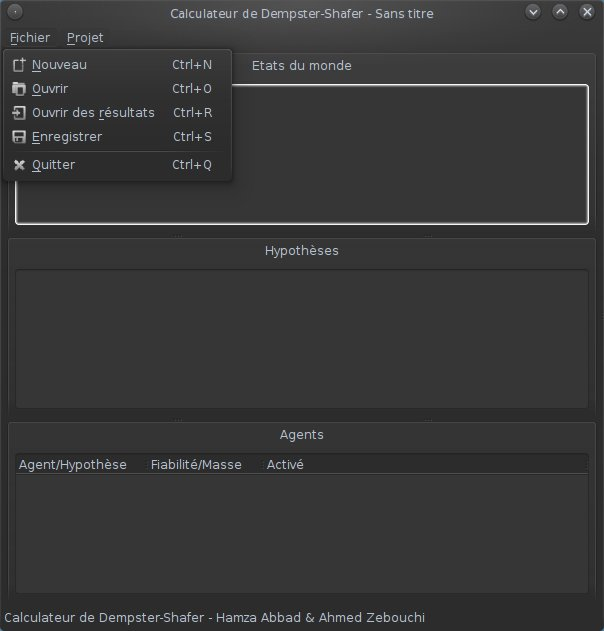
\includegraphics[width=\textwidth]{Inetrface_principale_menu_fichier}
\caption{Le menu \textbf{Fichier}}
\end{subfigure}
\hfill
\begin{subfigure}{0.49\textwidth}
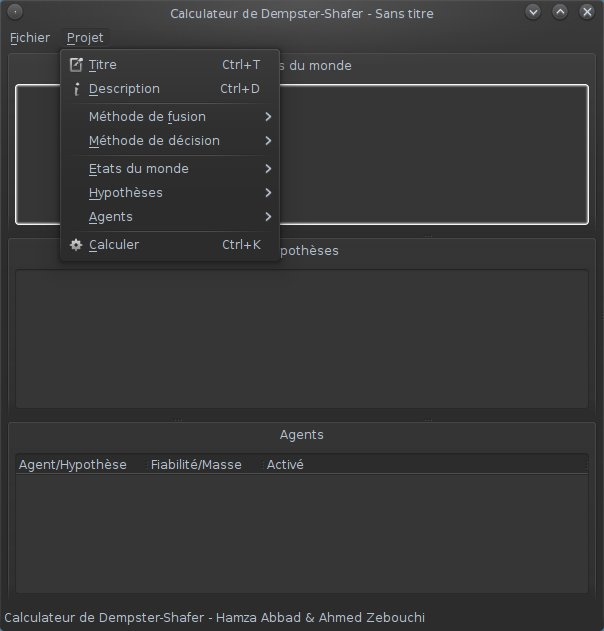
\includegraphics[width=\textwidth]{Inetrface_principale_menu_projet}
\caption{Le menu \textbf{Projet}}
\end{subfigure}
\caption{L'interface principale du \appname}
\end{figure}

Les états du monde, les hypothèses et les agents doivent s'ajouter dans cet ordre à partir
de ce menu ou par un clic droit dans leurs champs. \`A partir de ce menu, l'utilisateur a la possibilité de sélectionner une
des méthodes de fusion: \textit{Dempster-Shafer}, \textit{Dubois-Prade}, \textit{Smets} ou
\textit{Yager}. Il peut aussi choisir la méthode de décision qui sera utilisée parmi les trois
suivantes: \textit{Optimiste}, \textit{Pessimiste} ou \textit{Pignistique}.

La première étape consiste à ajouter tous les états du monde. Ensuite, chaque fois qu'un ensemble d'états est sélectionné
l'hypothèse correspondante est établie.\\[1em]

\begin{figure}[H]
\begin{subfigure}{0.49\textwidth}
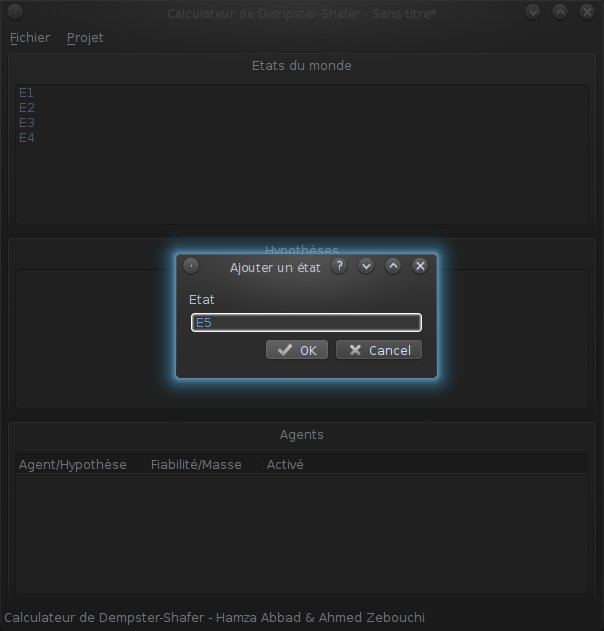
\includegraphics[width=\textwidth]{ajouter_etat}
\caption{Ajouter les états du monde}
\end{subfigure}
\hfill
\begin{subfigure}{0.49\textwidth}
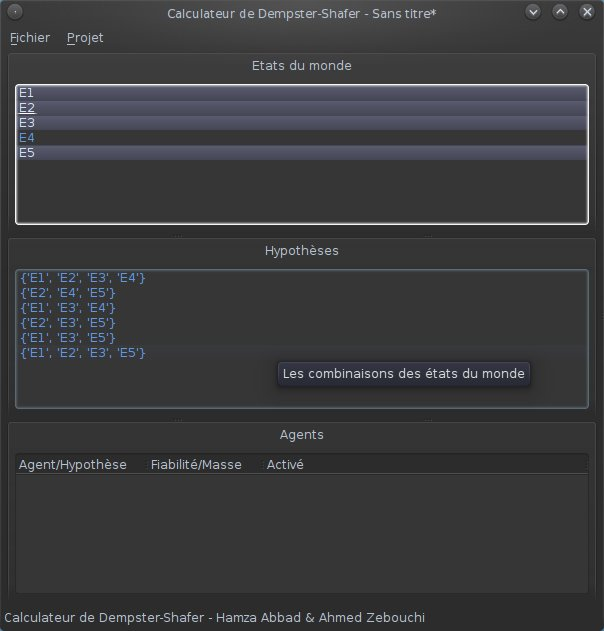
\includegraphics[width=\textwidth]{ajouter_hypothese}
\caption{Ajouter une hypothèse à partir des états}
\end{subfigure}
\caption{L'ajout des états du monde et les hypothèses}
\end{figure}

Par la suite, l'utilisateur doit procéder à l'ajout des agents. Chaque agent doit avoir un nom, un niveau de
fiabilité et un ensemble d'hypothèses tel que à chaque hypothèse est affectée une masse entre
$0$ et $1$.\\[1em]

\begin{figure}[H]
\begin{subfigure}{0.49\textwidth}
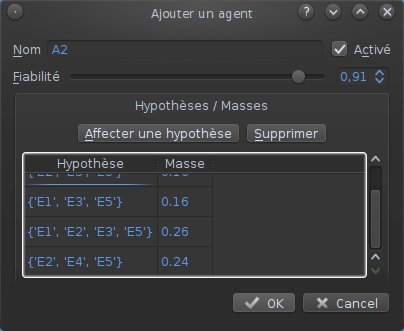
\includegraphics[width=\textwidth]{ajouter_agent}
\caption{Dialogue de l'ajout d'un agent}
\end{subfigure}
\hfill
\begin{subfigure}{0.49\textwidth}
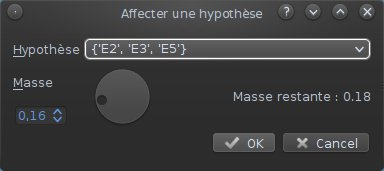
\includegraphics[width=\textwidth]{affecter_masse}
\caption{Dialogue de l'affectation d'une hypothèse}
\end{subfigure}
\caption{L'ajout d'un agent et l'affectation de ses hypothèses}
\end{figure}

Avant de passer au calcul, les données saisies doivent être enregistrées dans un fichier à l'aide de la fonctionnalité
\textbf{Enregistrer} ou \textbf{Enregistrer sous}. Il faut aussi choisir un nom et un emplacement pour le
fichier. Il aura par défaut l'extention \texttt{.dsti.xml}. Cette action est nécessaire car elle génère
le fichier d'entrée pour le noyau. Si cette étape est ignorée, le programme demandera de la faire avant de
continuer.\\[1em]

\begin{figure}[H]
\centering
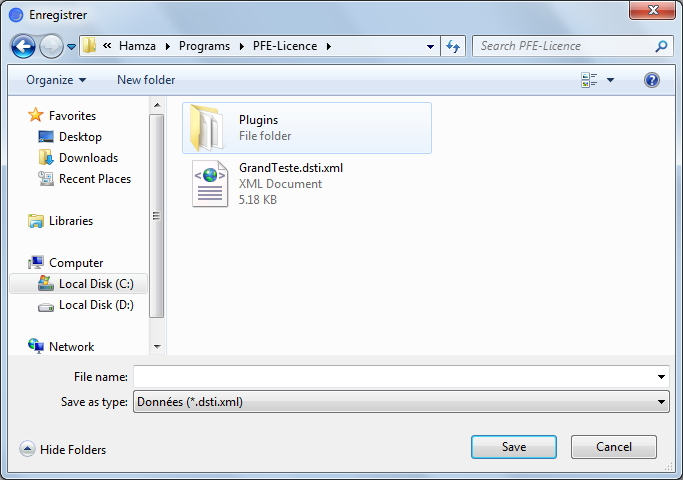
\includegraphics[width=0.8\textwidth]{Enregistrer}
\caption{Enregistrer les données}
\end{figure}

La dernière étape consiste à lancer le calcul. Cette étape risque de prendre un temps important si le nombre des états
du monde et/ou des agents est assez grand. Pour cela, un dialogue d'attente est affiché pendant l'exécution
du noyau en arrière-plan. L'utilisateur peut annuler cette opération à tout moment en cliquant sur le bouton
\emph{Annuler}.

Quand le calcul se termine, un dialogue contenant les informations du projet et tous les résultats sera affiché.
Les résultats sont obtenus par la lecture du fichier généré par le noyau qui a le même chemin que le fichier
sauvegardé, sauf qu'il porte l'extention \texttt{.dsto.xml}. Ce dialogue permet de rechercher une hypothèse en
tapant une partie de son nom dans la zone de texte qui contient le mot \emph{Rechercher}.
Les hypothèses qui correspondent à l'entrée de l'utilisateur sont sélectionnées afin de faciliter
la recherche. Il y a aussi un bouton permettant de créer un nouvel agent et de remplir ses hypothèses et ses masses
à partir de celles affichées. L'utilisateur doit introduire le nom de cet agent.

\begin{figure}[H]
\begin{subfigure}{0.39\textwidth}
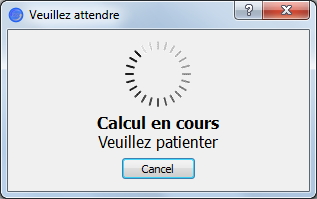
\includegraphics[width=\textwidth]{Dialogue_attente}
\caption{Dialogue d'attente}
\end{subfigure}
\hfill
\begin{subfigure}{0.59\textwidth}
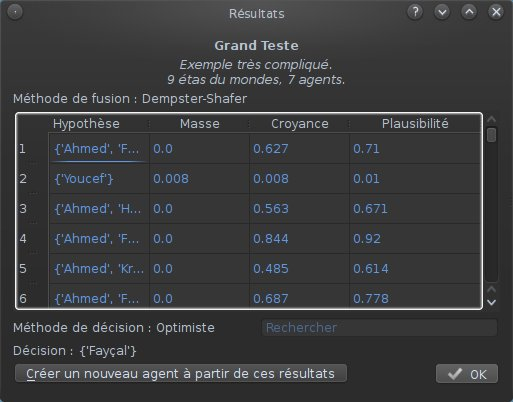
\includegraphics[width=\textwidth]{Dialogue_resultats}
\caption{Dialogue des résultats}
\end{subfigure}
\caption{Le calcul et l'affichage des résultats}
\end{figure}

Par la suite, les fichiers de données peuvent être accessibles en utilisant l'action \textbf{Ouvrir} à partir
du menu fichier. Les résultats peuvent être aussi affichés en ouvrant le fichier correspondant en utilisant l'action
\textbf{Ouvrir des résultats}.

\begin{figure}[H]
\begin{subfigure}{0.49\textwidth}
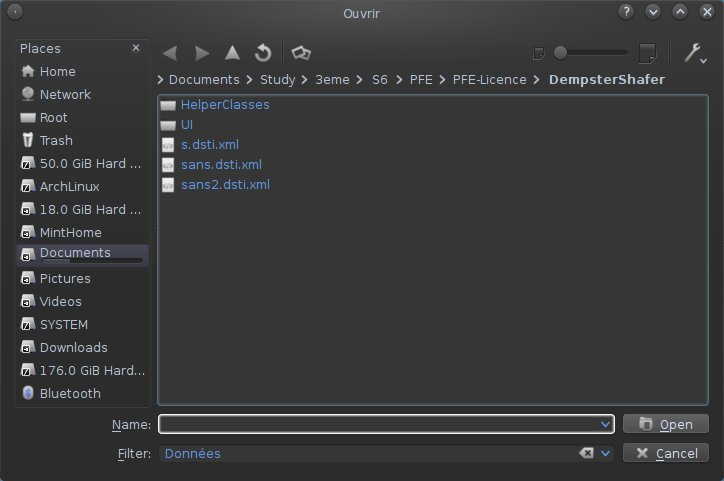
\includegraphics[width=\textwidth]{Ouvrir}
\caption{Dialogue d'ouverture d'un fichier de données}
\end{subfigure}
\hfill
\begin{subfigure}{0.49\textwidth}
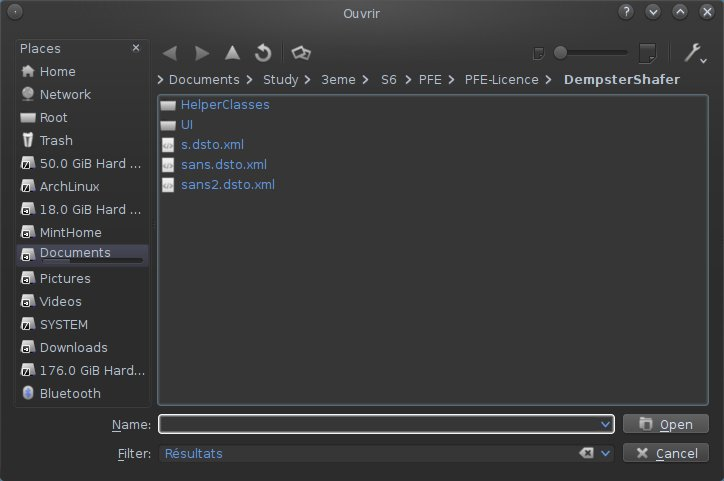
\includegraphics[width=\textwidth]{Ouvrir_resultats}
\caption{Dialogue d'ouverture de résultats}
\end{subfigure}
\caption{Les dialogues de l'ouverture d'un fichier}
\end{figure}

\section{La \platformename}

Ce programme est une interface composée de plusieurs panneaux et chaque panneau est accessible
à partir de son titre dans la barre des onglets. Un panneau comporte une ou plusieurs interfaces pour
un ou plus d'un programme externe.  La \platformename est facilement extensible; pour ajouter un nouveau
panneau dans cette interface il suffit de créer une classe personnalisée qui dérive de la classe
\mbox{\texttt{javax.swing.JPanel}} dans le paquet \texttt{Plugins}. Jusqu'à présent, la \platformename
contient quatre onglets : \textit{Imprécision}, \textit{Décision}, \textit{Incertain}
et \textit{Tools}.

Dans le panneau \textit{Imprécision} il y a un bouton pour lancer la \textbf{Fuzzy Logic Toolbox} qui est une
bibliothèque de \textit{MATLAB} avec une interface graphique intégrée facilitant l'exploitation directe
de la bibliothèque.

\begin{figure}[H]
\centering
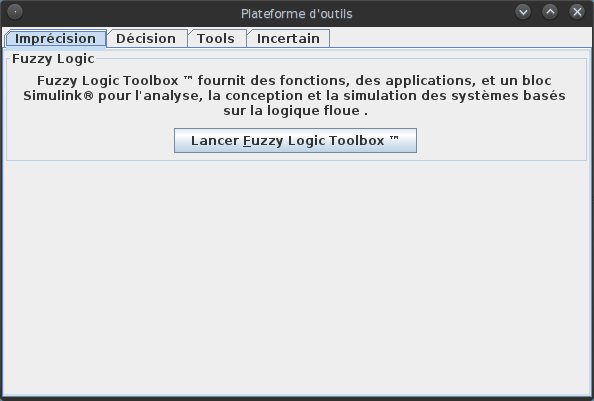
\includegraphics[width=0.7\textwidth]{Imprecision}
\caption{Le panneau \textbf{Imprécision}}
\end{figure}

Le panneau \textit{Décision} contient deux parties, l'une appelée \textit{Logique}
contenant un bouton pour exécuter l'application \textbf{DecPos} qui permet de calculer la décision optimale dans
le cas pessimiste ou optimiste et d'effectuer autres opérations sur les bases possibilistes; l'autre qui
s'appelle \textit{Graphique} qui contient un bouton pour exécuter l'application \textbf{GraphViz02} pour
le traitement des graphes de décision.

\begin{figure}[H]
\begin{subfigure}{0.49\textwidth}
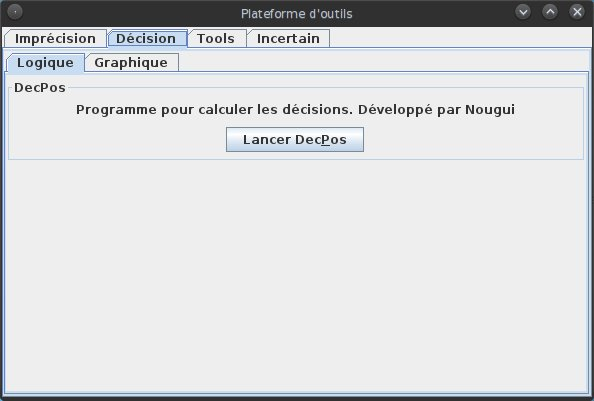
\includegraphics[width=\textwidth]{Decision_logique}
\caption{La partie \textbf{Logique}}
\end{subfigure}
\hfill
\begin{subfigure}{0.49\textwidth}
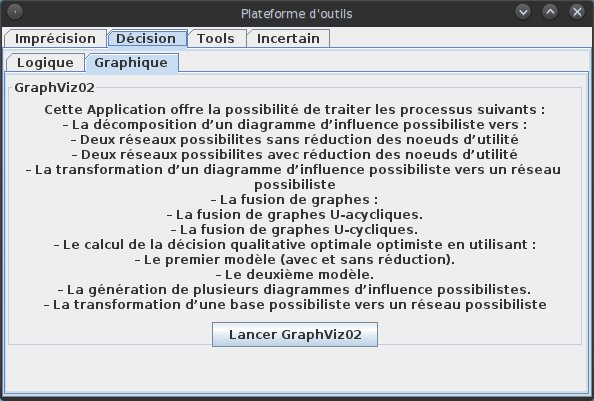
\includegraphics[width=\textwidth]{Decision_graphique}
\caption{La partie \textbf{Graphique}}
\end{subfigure}
\caption{Le panneau \textbf{Décision}}
\end{figure}

\vspace*{1.5em}
Le panneau \textit{Incertain} regroupe les interfaces nécessaires pour dessiner un graphe orienté sans
cycles de nature BNT ou PNT et pour modifier ses paramètres après la validation. Il y a un bouton \textbf{Ajouter un noeud}
permettant d'ajouter un nouveau nœud isolé. Les noeuds doivent être reliés par des arcs qui sont créés par le
glissement du curseur à partir d'un noeud et le relâchement dans un autre. Ensuite, l'utilisateur doit valider le graphe
en utilisant le bouton \textbf{Valider} et puis il doit changer les paramètres de chaque noeud et spécifier la vraissemblance,
le noeud observé, et ajouter les évidences. Enfin il peut générer un script \textit{MATLAB} et de l'exécuter en cliquant
sur le bouton \textbf{Calculer}.
\vspace*{3em}

\begin{figure}[H]
\centering
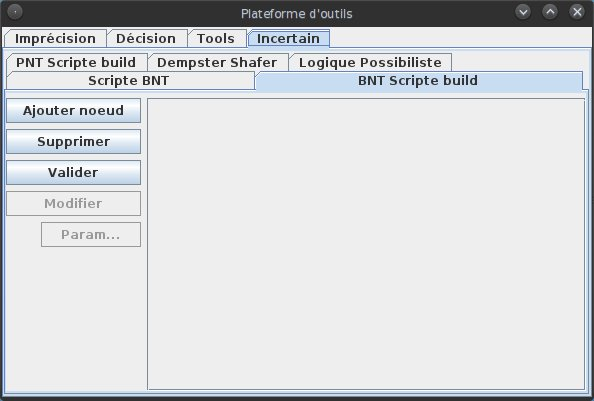
\includegraphics[width=0.7\textwidth]{Incertain_BNT_graphe}
\caption{L'interface du graphe BNT}
\end{figure}
\vspace*{2em}

Dans le même panneau, il y a aussi un panneau interne qui porte le nom \textit{Dempster-Shafer} pour exécuter
notre application \appname qui a été présentée auparavant. Le dernier panneau est celui de \textit{Logique possibiliste}.
Il représente une interface pour un ensemble des programmes qui seront exécutés en série. Il permet de spécifier le nombre
de noeuds dans un graphe possibiliste et le nombre maximal de parents pour chaque noeud, ainsi que le nombre de propositions
(1 ou 2). Le programme génère un graphe aléatoire par lancement d'un script \textit{MATLAB} suivi par deux programmes
\texttt{passage} et \texttt{inference}. Enfin, il affiche les résultats pour l'utilisateur.

\begin{figure}[H]
\begin{subfigure}{0.49\textwidth}
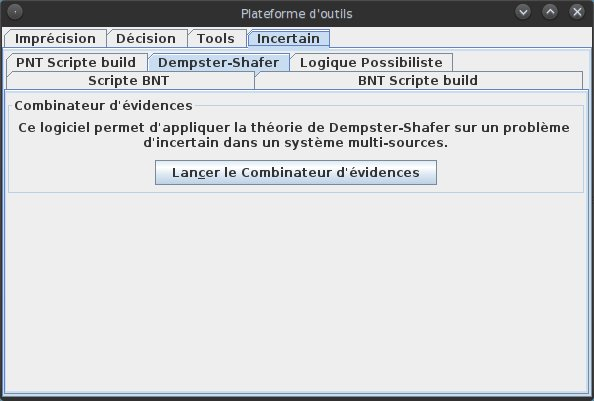
\includegraphics[width=\textwidth]{Incertain_DS}
\caption{Le panneau interne \textbf{Dempster-Shafer}}
\end{subfigure}
\begin{subfigure}{0.49\textwidth}
\hfill
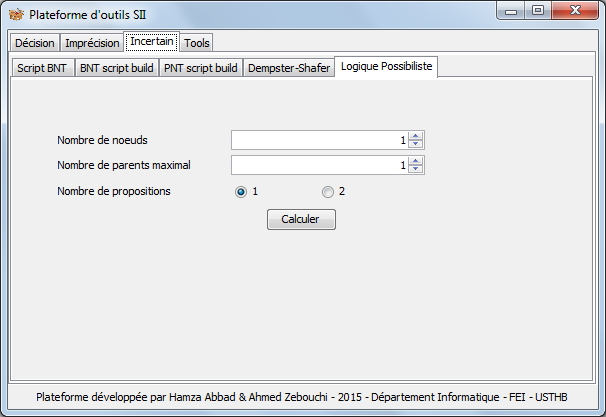
\includegraphics[width=\textwidth]{Incertain_LP}
\caption{Le panneau interne \textbf{Logique possibiliste}}
\end{subfigure}
\caption{Le panneau \textbf{Incertain}}
\end{figure}

Le dernier panneau \textit{Tools} contient deux interfaces pour utiliser le logiciel \textbf{UBCSAT}, la
première pour calculer le SAT et la deuxième pour le Weighted Max SAT. L'utilisateur doit introduire les formules
logiques sous forme FND\footnote{Forme normale disjonctive}.

\begin{figure}[H]
\centering
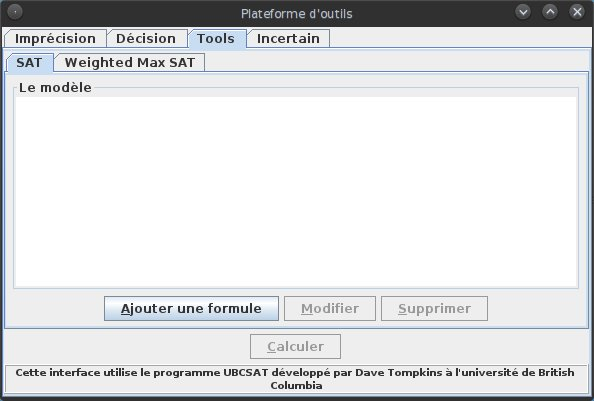
\includegraphics[width=0.7\textwidth]{Tools_SAT}
\caption{Le panneau \textbf{Tools}}

\end{figure}
\vspace*{-2em}
\phantomsection
\addcontentsline{toc}{section}{Conclusion}
\section*{Conclusion}

Nous avons présenté globalement ce que nous avons réalisé dans notre projet. Nous avons commencé par une
présentation détaillée de notre application \appname que nous avons entièrement développée, et puis, nous
avons montré les différentes tâches qui peuvent être réalisées à travers notre interface \platformename.

\phantomsection
\addcontentsline{toc}{chapter}{Conclusion générale}
\chapter*{Conclusion générale}

Sur le plan théorique, notre travail s'est situé dans le cadre du traitement des connaissances incertaines,
principalement sur la fusion de croyances sous la théorie de Dempster-Shafer. Nous avons également pris connaissances
de plusieurs théories de l'incertain et de l'imprécision.

Nous avons donc fait une étude pour comprendre et pouvoir exposer les notions générales de la théorie de Dempster-Shafer,
en expliquant les fonctions de croyance, les règles de combinaisons et les règles de décision. 
Nous avons aussi conçu et implémenté les algorithmes nécessaires pour l'exploitation complète de cette théorie. De plus,
nous avons présenté brièvement les autres théories de l'incertain qui sont situées dans le même domaine que notre sujet.

Sur le plan pratique, nous avons réalisé deux applications. La première est un logiciel qui permet la représentation,
puis la résolution d'un problème d'incertitude dans le cas d'une expertise multiple en appliquant la théorie de
Dempster-Shafer.
La deuxième application est une plateforme qui fait appel à différent outils qui implémentent des théories de
l'incertain et de la logique floue.

Comme perspectives, il serait intéressant de modifier notre plateforme en ajoutant des interfaces pour d'autres outils
manquants dans cette version, ou même de supprimer les existantes s'ils ne seront plus utiles. Pour cela, nous avons créé
la plateforme de façon à faciliter son extension.

Nous souhaitons que notre travail soit bénéfique pour notre université et nous espérons qu'il sera utilisé dans autres
établissements. En effet, il peut fournir une aide importante pour les personnes spécialisées dans le domaine de
la représentation et le raisonnement sur les connaissances incertaines.
\bibliographystyle{babplain}
\phantomsection
\addcontentsline{toc}{chapter}{Bibliographie}
\bibliography{bibliographie}
\end{document}          
